% !TEX spellcheck = en_US
% !TeX root = main.tex


\noindent Extensive experiments are performed to evaluate the performance of our FlowKG by answering the following research questions:

\begin{itemize}
	\item \textbf{RQ1:} How does FlowKG perform compared to state-of-the-art recommendation baselines?
	\item \textbf{RQ2:} How do key components contribute to the model's effectiveness, and how do critical hyperparameters influence its performance?
	\item \textbf{RQ3:} Can FlowKG effectively mitigate the impact of knowledge noise and maintain robustness across varying data distributions?
	\item \textbf{RQ4:} How does the computational efficiency (in terms of training time and model parameters) of FlowKG compare to state-of-the-art baselines?
	\item \textbf{RQ5:} Can the learned representations visually demonstrate the manifold refinement process and semantic separation of items?
\end{itemize}

\subsection{Experimental Settings}

\subsubsection{\textbf{Datasets}}
To ensure comprehensive evaluation across diverse domains and sparsity levels, we utilize four benchmark datasets: MIND~\cite{wu2020mind} (News), MovieLens-1M~\cite{harper2015movielens} (Movies), Last-FM~\cite{cantador2011second} (Music), and Yelp\footnote{\url{https://www.yelp.com/dataset}} (Business). To guarantee data quality and fairness, we employ a unified KG construction approach and apply a 10-core filtering setting~\cite{jiang2024diffkg,li2025mask}. Consistent with standard protocols, we adopt an 80:10:10 split for training, validation, and testing, respectively. Table~\ref{tab:data statistics} summarizes the detailed statistics of the User-Item Graphs and Knowledge Graphs for all datasets.

\subsubsection{\textbf{Evaluation Protocols}}
We implement a comprehensive all-ranking strategy~\cite{ren2024representation,wang2019kgat,yang2023knowledge} to evaluate recommendation performance. To strictly assess the quality of Top-$N$ recommendations, we employ two widely adopted metrics: Recall@20 and NDCG@20. Recall measures the proportion of relevant items successfully retrieved, while NDCG evaluates the ranking quality by assigning higher scores to hits positioned near the top of the list.

\subsubsection{\textbf{Baselines for Comparison}}
To benchmark the effectiveness of FlowKG, we compare it against a diverse set of state-of-the-art knowledge-aware recommenders.

\noindent\textbf{Conventional Embedding and Translation-based Methods.}
\begin{itemize}
	\item \textbf{FM}~\cite{rendle2011fast} is a classic embedding-based method that models high-order feature interactions via factorized parameters to incorporate context information as auxiliary features.
	\item \textbf{CKE}~\cite{zhang2016collaborative} integrates collaborative filtering with structural, textual, and visual knowledge embeddings extracted via TransR and auto-encoders.
	\item \textbf{KTUP}~\cite{cao2019unifying} employs a translation-based approach to jointly learn recommendation and knowledge graph completion tasks, transferring relational information to model user preferences.
\end{itemize}

\noindent\textbf{Propagation-based Graph Neural Network Methods.}
\begin{itemize}
	\item \textbf{KGAT}~\cite{wang2019kgat} applies graph neural networks with an attention mechanism to recursively propagate embeddings and model high-order connectivities within a collaborative knowledge graph.
	\item \textbf{KGIN}~\cite{wang2021learning} explores latent user intents behind interactions by aggregating relational paths and modeling intents as attentive combinations of KG relations.
	\item \textbf{LECF}~\cite{huang2024lorentz} leverages hyperbolic geometry to capture hierarchical structures in knowledge graphs and ensures Lorentz group equivariance during the message propagation process.
\end{itemize}


\setlength{\tabcolsep}{3pt}
\begin{table}[t]
	\small
	\centering
	\caption{Statistics of the experimental datasets.}
	\label{tab:data statistics}
		\begin{tabular}{lrrrr}
			\toprule
			Statistics & MIND & ML-1M & Last-FM & Yelp \\
			\midrule
			\# Users & 100,000 & 6,036 & 1,815 & 16,308 \\
			\# Items & 30,577 & 2,347 & 3,846 & 11,516 \\
			\# Interactions & 2,975,319 & 301,509 & 17,523 & 159,302 \\
			\midrule
			\multicolumn{5}{c}{Knowledge Graph} \\
			\midrule
			\# Entities & 49,545 & 6,729 & 9,366 & 24,176 \\
			\# Relations & 512 & 12 & 60 & 42 \\
			\# Triples & 297,058 & 38,346 & 19,586 & 47,204 \\
			\bottomrule
		\end{tabular}
\end{table}

\noindent\textbf{Self-Supervised Contrastive Learning Frameworks.}
\begin{itemize}
	\item \textbf{KGIC}~\cite{zou2022improving} introduces a multi-level interactive contrastive learning mechanism that contrasts local and non-local graph views to mitigate data sparsity and noise.
	\item \textbf{KGRec}~\cite{yang2023knowledge} proposes a self-supervised rationalization framework that identifies informative knowledge connections through generative masking and contrastive alignment tasks.
	\item \textbf{LightKG}~\cite{li2025lightkg} features a simplified GNN architecture with linear aggregation and an efficient contrastive layer to address data sparsity and computational complexity.
\end{itemize}

\noindent\textbf{Generative and Diffusion-based Recommendation Models.}
\begin{itemize}
	\item \textbf{DiffKG}~\cite{jiang2024diffkg} integrates a generative diffusion model with data augmentation to reconstruct the knowledge graph and align semantic signals with collaborative data.
	\item \textbf{KMDCL}~\cite{li2025mask} combines mask-based diffusion models with contrastive learning to adaptively generate denoised views guided by user intentions for robust representation learning.
\end{itemize}


%\subsubsection{\textbf{Parameter Settings.}}
%Our baseline settings are consistent with our model parameter configurations, and any additional parameters for baselines follow the default settings reported in their respective papers or public implementations.
%We employ a fixed learning rate of $1e^{-4}$, a batch size of 1024, and a fixed embedding dimension of 64. The FlowKG framework was optimized using the Adam optimizer, with model parameters initialized via Xavier initialization.
%
%Regarding the model-specific hyperparameters, we conducted a grid search to identify optimal configurations.
%\begin{itemize}
%	\item \textbf{Dual-View Encoder:} The number of layers for the collaborative view ($L_{cf}$) and the semantic view ($L_{kg}$) are tuned independently within the range of $\{1, 2, 3\}$. The noise perturbation magnitude $\epsilon$ is searched in $\{0.05, 0.1, 0.2, 0.5\}$.
%	\item \textbf{Structure Learning:} For the entropy-guided structure learning module, both the retention rate $\rho$ and the balance factor $\alpha$ are tuned in the range of $\{0.1, 0.2, \dots, 0.9\}$.
%	\item \textbf{Flow Matching:} The time step embedding size is fixed to 10. The starting time step of the evolution trajectory, denoted as $t_{\text{start}}$, is tuned in the range of $\{0.1, 0.2, \dots, 0.9\}$. Regarding the Euler integration strategy, we explore the integration steps $N$ in the range of $\{1, \dots, 5\}$ during the inference phase to balance efficiency and performance.
%	\item \textbf{Loss and Regularization:} The contrastive loss weight $\lambda_1$ is optimized in $\{0.0, 0.2, \dots, 1.0\}$, and the flow matching loss weight $\lambda_2$ is tuned in $\{1, 2, 5, 10, 20\}$. The temperature hyperparameter $\tau$ is searched in $\{0.1, 0.2, \dots, 1.0\}$. Notably, for datasets exhibiting a preference for higher temperatures, we further investigate the asymptotic limit where $\tau \to \infty$, implemented as the Mean Difference (MD) loss, to evaluate the effectiveness of global alignment in the representation space. The $L_2$ regularization coefficient $\lambda_{reg}$ is searched in $\{1e^{-7}, 1e^{-6}, 1e^{-5}\}$.
%\end{itemize}
%These parameter configurations establish an initial tuning baseline, which is further refined based on the validation performance. We implemented our model using PyTorch on an NVIDIA RTX 4090 GPU.
%\begin{table}[t]
%	\centering
%	\caption{Statistics of the experimental datasets.}
%	\label{tab:data statistics}
%	\renewcommand{\arraystretch}{1.2}
%	\setlength{\tabcolsep}{2pt}
%	\begin{tabular}{lcccc}
	%		\toprule
	%		Statistics & MIND & MovieLens-1M & Last-FM & Yelp \\
	%		\midrule
	%		Users        & 100,000 & 6,036 & 1,815 & 16,308 \\
	%		Items        & 30,577  & 2,347 & 3,846 & 11,516 \\
	%		Interactions & 2,975,319 & 301,509 & 17,523 & 159,302 \\
	%		\midrule
	%		Entities     & 49,545 & 6,729 & 9,366 & 24,176 \\
	%		Relations    & 512    & 12    & 60    & 42 \\
	%		KG triples   & 297,058 & 38,346 & 19,586 & 47,204 \\
	%		\bottomrule
	%	\end{tabular}
%\end{table}


\subsubsection{\textbf{Parameter Settings}}
We implement FlowKG and all baselines using PyTorch on an NVIDIA RTX 4090 GPU. For a fair comparison, we fix the embedding dimension to 64, the batch size to 1024, and the learning rate to $1e^{-4}$, optimizing the model via Adam~\cite{kingma2014adam} with Xavier initialization~\cite{xavier2007unravelling}. Baseline hyperparameters follow the optimal settings reported in their respective papers. For FlowKG, we determine the optimal hyperparameters via grid search on the validation set. Specifically, the layer depths for collaborative and semantic views ($L_{cf}, L_{kg}$) are tuned in $\{1, 2, 3\}$, and the noise perturbation $\epsilon$ is searched in $\{0.05, \dots, 0.5\}$. The structure learning parameters $\rho$ and $\alpha$ are adjusted within $[0.1, 0.9]$. For the Flow Matching module, we set the time step embedding size to 10 and tune the start time $t_{\text{start}}$ in $[0.1, 0.9]$. Regarding the optimization objectives, the user-side and item-side contrastive loss weights $\lambda_{u}$ and $\lambda_{i}$ are tuned in $[0.0, 1.0]$, and the flow matching loss weight $\lambda_{\text{fm}}$ is tuned in $\{1, \dots, 20\}$. The temperature $\tau$ is searched in $\{0.1, \dots, 1.0\}$ (including the MD loss limit), and the $\ell_2$ regularization coefficient $\lambda_{\text{reg}}$ is selected from $\{1e^{-7}, 1e^{-6}, 1e^{-5}\}$. During inference, the Euler integration steps $N$ are selected from $\{1, \dots, 5\}$ to balance efficiency and accuracy.

\setlength{\tabcolsep}{6pt}
\begin{table*}[t]
	\small
	\centering
	\caption{Performance comparison on MIND, MovieLens-1M (ML-1M), Last-FM, and Yelp datasets. The best results are highlighted in \textbf{bold}, and the second-best results are \underline{underlined}. $^*$ indicates statistically significant improvements by paired t-test with $p\text{-value} < 0.01$.}
	\label{tab:overall_performance}
		\begin{tabular}{l|cc|cc|cc|cc}
			\toprule
			\multirow{2}{*}{Model} 
			& \multicolumn{2}{c|}{MIND} 
			& \multicolumn{2}{c|}{MovieLens-1M} 
			& \multicolumn{2}{c|}{Last-FM}
			& \multicolumn{2}{c}{Yelp} \\
			
			\cmidrule(lr){2-3} \cmidrule(lr){4-5} \cmidrule(lr){6-7} \cmidrule(lr){8-9}
			
			& Recall@20 & NDCG@20
			& Recall@20 & NDCG@20
			& Recall@20 & NDCG@20
			& Recall@20 & NDCG@20 \\
			\midrule
			
			FM
			& 0.0237 & 0.0163 & 0.1486 & 0.0798 & 0.1742 & 0.1231 & 0.0617 & 0.0363 \\
			CKE
			& 0.0387 & 0.0247 & 0.1842 & 0.1276 & 0.2651 & 0.1604 & 0.0639 & 0.0407 \\
			KTUP
			& 0.0362 & 0.0302 & 0.2094 & 0.1741 & 0.2042 & 0.1635 & 0.0663 & 0.0412 \\
			KGAT
			& 0.0340 & 0.0287 & 0.2132 & 0.1797 & 0.2051 & 0.1671 & 0.0698 & 0.0426 \\
			KGIN
			& 0.0357 & 0.0225 & 0.2269 & 0.1859 & 0.2764 & 0.1758 & 0.0715 & 0.0438 \\
			LECF
			& 0.0387 & 0.0272 & 0.2348 & 0.1946 & 0.2896 & 0.1773 & 0.0729 & 0.0453 \\
			KGIC
			& 0.0525 & 0.0307 & 0.2014 & 0.1671 & 0.2901 & 0.1805 & 0.0758 & 0.0461 \\
			KGCL
			& 0.0399 & 0.0274 & 0.2315 & 0.1910 & 0.2810 & 0.1795 & 0.0755 & 0.0465 \\
			KGRec
			& 0.0439 & 0.0319 & 0.2194 & 0.1901 & 0.2742 & 0.1556 & 0.0783 & 0.0476 \\
			LightKG
			&0.0445 & 0.0276 & \underline{0.3305} & \underline{0.3132} & \underline{0.4017} & \underline{0.2430} &0.0754 & 0.0458\\		
			DiffKG
			& 0.0615 & 0.0389 & 0.3064 & 0.2875 & 0.3593 & 0.2091 & 0.0935 & 0.0518 \\
			KMDCL
			& \underline{0.0646} & \underline{0.0419} & 0.3269 & 0.3059 & 0.3806 & 0.2205 & \underline{0.0991} & \underline{0.0546} \\
			
			\hline
			
			\rule{0pt}{2ex}\textbf{FlowKG} 
			& \textbf{0.0937}$^{*}$ & \textbf{0.0607}$^{*}$ 
			& \textbf{0.3517}$^{*}$ & \textbf{0.3283}$^{*}$ 
			& \textbf{0.4106}$^{*}$ & \textbf{0.2509}$^{*}$ 
			& \textbf{0.1232}$^{*}$ & \textbf{0.0691}$^{*}$ \\
			\bottomrule
		\end{tabular}
\end{table*}

\begin{table}[!tbp]
	\small
	\centering
	\setlength{\tabcolsep}{1.8pt}
	\caption{Ablation study of FlowKG on three representative datasets. The full four-dataset results are reported in Appendix~\ref{app:full_ablation}. The best results are highlighted in bold.}
	\label{tab:ablation}
	\begin{tabular}{l|cc|cc|cc}
		\toprule
		\multirow{2}{*}{Variants}
		& \multicolumn{2}{c|}{MIND}
		& \multicolumn{2}{c|}{ML-1M}
		& \multicolumn{2}{c}{Last-FM} \\
		\cmidrule(lr){2-3} \cmidrule(lr){4-5} \cmidrule(lr){6-7}
		& R@20 & N@20 & R@20 & N@20 & R@20 & N@20 \\
		\midrule
		 w/o ESL & 0.0930 & 0.0601 & 0.3474 & 0.3249 & 0.4073 & 0.2473 \\
		 w/o DVE & 0.0886 & 0.0565 & 0.3258 & 0.3072 & 0.3990 & 0.2445 \\
		 w/o FM  & 0.0764 & 0.0510 & 0.3374 & 0.3131 & 0.3892 & 0.2385 \\
		 w/o CL  & 0.0612 & 0.0396 & 0.3242 & 0.3059 & 0.3862 & 0.2200 \\
		\hline
		\rule{0pt}{2ex}Full Model & \textbf{0.0937} & \textbf{0.0607} & \textbf{0.3517} & \textbf{0.3283} & \textbf{0.4106} & \textbf{0.2509} \\
		\bottomrule
	\end{tabular}
\end{table}

\subsection{Performance Comparison (RQ1)}

Table~\ref{tab:overall_performance} demonstrates that FlowKG consistently achieves state-of-the-art performance, significantly outperforming all baselines across datasets. Early GNNs (e.g., KGAT) capture connectivity but suffer from noise propagation. Subsequent CL methods (e.g., KGRec, LightKG) improve robustness via self-supervision; however, they remain constrained by cascaded architectures or lack effective handling of underlying structural noise. Furthermore, we observe that LightKG delivers outstanding performance on dense datasets (ML-1M, Last-FM) via simplification; yet, it exhibits significant degradation on interaction-sparse datasets (MIND), indicating insufficient capability to capture scarce collaborative signals. While generative baselines like KMDCL show promise, they rely on stochastic diffusion processes.

In contrast, FlowKG establishes a substantial margin over the strongest baseline KMDCL, achieving remarkable improvements particularly on the sparse MIND and Yelp datasets. This superiority stems from two fundamental designs: \begin{itemize} \item \textbf{Direct Latent Refinement.} Unlike methods that diffuse graph structures or rely on stochastic sampling, FlowKG employs Flow Matching to construct deterministic ODE paths directly in the continuous representation space. This allows for a more direct and stable evolution of embeddings from noise to high-quality semantic manifolds. \item \textbf{Pre-encoding Structural Purification.} Addressing the structural blindness of previous works, our Entropy-Guided module combines structural priors with learned semantic posteriors to assess triplet quality before encoding. This dual-scoring approach ensures the model learns from a purified semantic view, effectively preventing the ``garbage-in, garbage-out'' issue inherent in cascaded architectures. \end{itemize}

\begin{figure}[t]
	\centering
	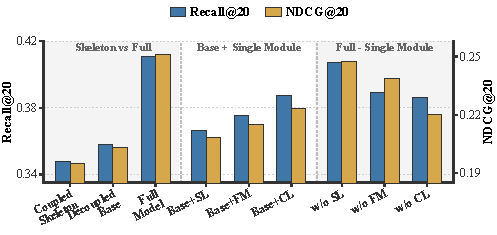
\includegraphics[width=\columnwidth]{image/ablation_chart_lastfm_unified}
	\caption{In-depth mechanism analysis on Last-FM, illustrating architecture evolution, additive gains, and subtractive impacts of key components.}
	\label{fig:ablation_chart_lastfm}
\end{figure}

\begin{figure*}[t] % 关键点：figure*
	\centering
	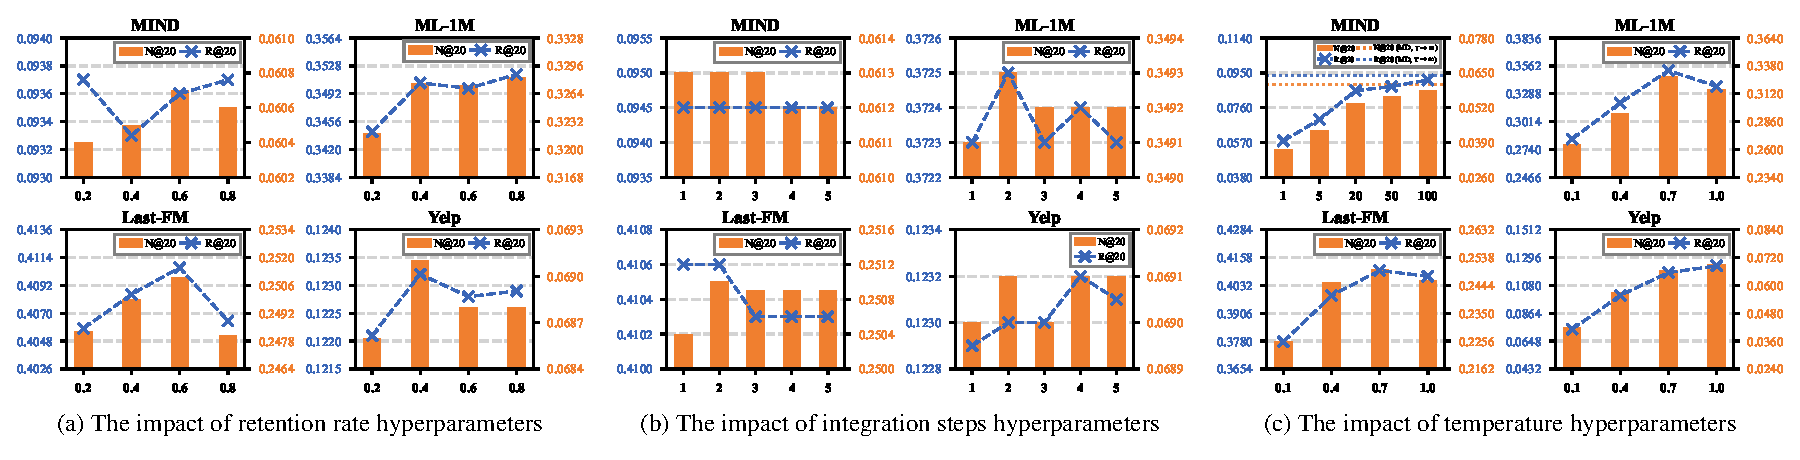
\includegraphics[width=1\textwidth]{image/hyperparameter_grid.pdf}
	\caption{Sensitivity analysis of key hyperparameters across four datasets, illustrating the impact of structure retention rate $\rho$, integration steps $N$, and contrastive temperature $\tau$. Dashed lines denote the theoretical performance limit using Mean Difference (MD) loss as $\tau \to \infty$.}
	\label{fig:hyperparameter}
\end{figure*}

\begin{figure}[t]
	\centering
	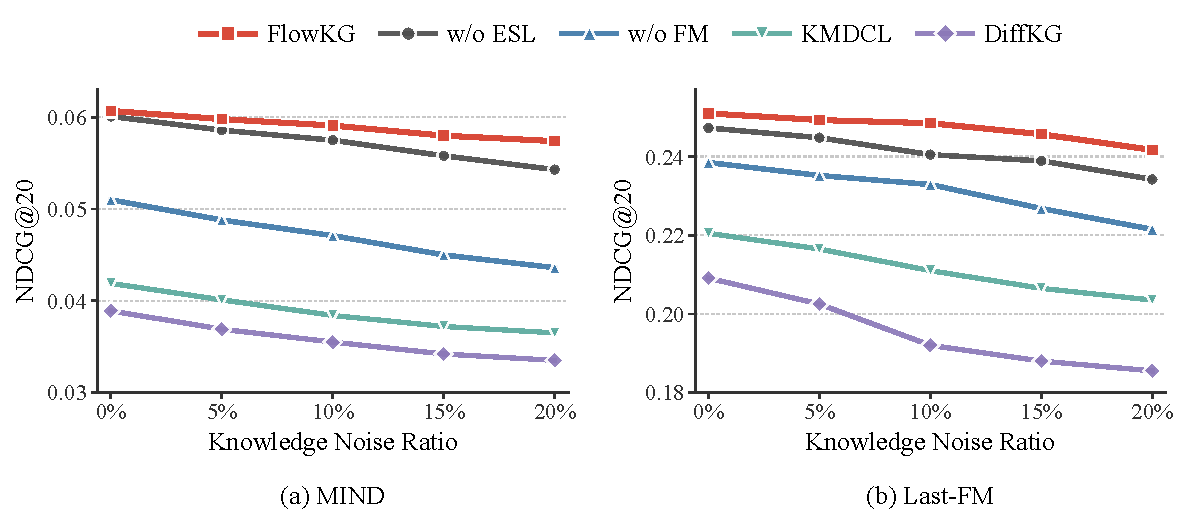
\includegraphics[width=\columnwidth]{image/noise_robustness}
	\caption{NDCG@20 under increasing knowledge noise ratios on MIND and Last-FM. The full FlowKG model is compared with its variants and representative baselines.}
	\label{fig:noise_robustness}
\end{figure}

\begin{figure}[t]
	\centering
	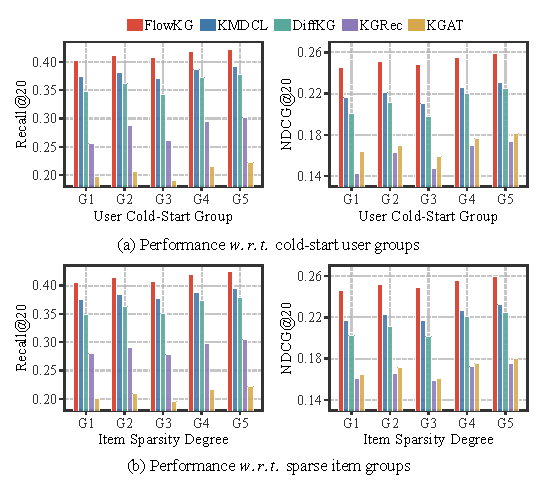
\includegraphics[width=\columnwidth]{image/lastfm_sparsity_metrics}
	\caption{Performance comparison across different user and item sparsity groups on Last-FM under NDCG@20 and Recall@20.}
	\label{fig:lastfm_sparsity_metrics}
\end{figure}

\begin{figure*}[t] % 星号 * 表示横跨双栏，[t] 表示通常建议放在页面顶部
	\centering
	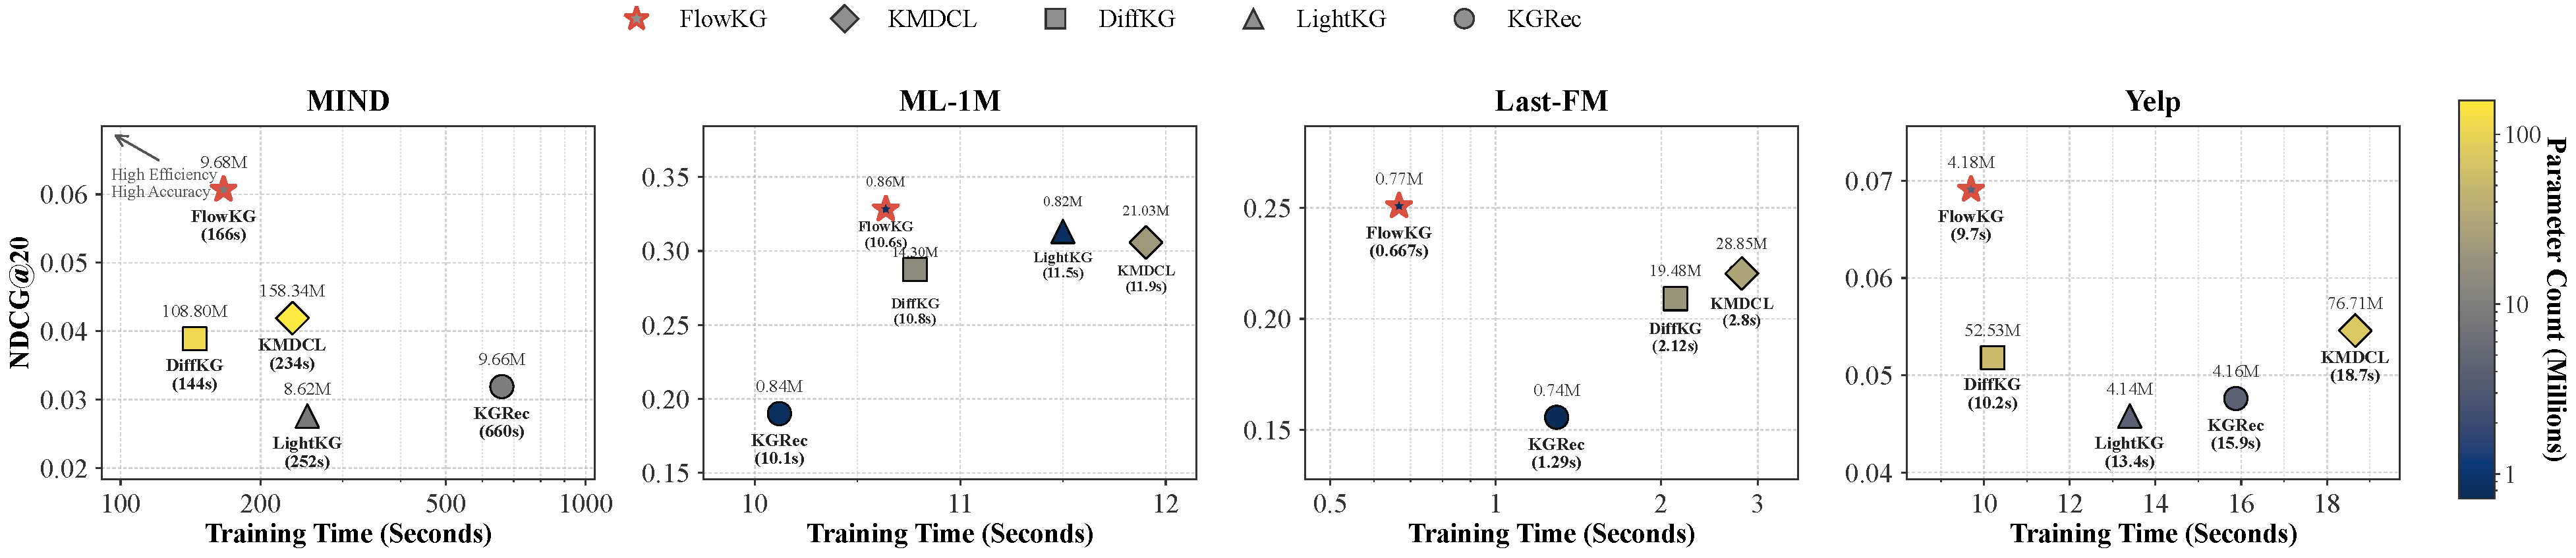
\includegraphics[width=1\textwidth]{image/efficiency_pareto.pdf} 
	% 使用 \textwidth 而不是 \columnwidth，因为你要跨越两栏
	\caption{Analysis of the trade-off between recommendation performance (NDCG@20) and training efficiency. The color intensity represents the model parameter scale, where FlowKG achieves the Pareto optimal balance across all datasets.}
	\label{fig:efficiency_pareto}
\end{figure*}

\iffalse
\begin{table}[t]
	\centering
	\caption{Tabular summary of the efficiency-performance trade-off in Figure~\ref{fig:efficiency_pareto}. Params denotes parameter count in millions, and Time denotes seconds per epoch.}
	\label{tab:efficiency_pareto}
	\scriptsize
	\setlength{\tabcolsep}{3.0pt}
	\renewcommand{\arraystretch}{1.05}
	\resizebox{\columnwidth}{!}{
		\begin{tabular}{llcccc}
			\toprule
			Methods & Component & MIND & ML-1M & Last-FM & Yelp \\
			\midrule
			\multirow{3}{*}{FlowKG}
			& NDCG@20 & \textbf{0.0607} & \textbf{0.3283} & \textbf{0.2509} & \textbf{0.0691} \\
			& Params (M) & 9.68 & 0.86 & 0.77 & 4.18 \\
			& Time (s) & 166.5 & 10.6 & 0.667 & 9.7 \\
			\midrule
			\multirow{3}{*}{KMDCL}
			& NDCG@20 & 0.0419 & 0.3059 & 0.2205 & 0.0546 \\
			& Params (M) & 158.34 & 21.03 & 28.85 & 76.71 \\
			& Time (s) & 234.0 & 11.9 & 2.8 & 18.7 \\
			\midrule
			\multirow{3}{*}{DiffKG}
			& NDCG@20 & 0.0389 & 0.2875 & 0.2091 & 0.0518 \\
			& Params (M) & 108.80 & 14.30 & 19.48 & 52.53 \\
			& Time (s) & 144.3 & 10.8 & 2.12 & 10.2 \\
			\midrule
			\multirow{3}{*}{LightKG}
			& NDCG@20 & 0.0276 & 0.3132 & 0.2430 & 0.0458 \\
			& Params (M) & 8.62 & 0.82 & 0.72 & 4.14 \\
			& Time (s) & 252.0 & 11.5 & 0.2 & 13.4 \\
			\midrule
			\multirow{3}{*}{KGRec}
			& NDCG@20 & 0.0319 & 0.1901 & 0.1556 & 0.0476 \\
			& Params (M) & 9.66 & 0.84 & 0.74 & 4.16 \\
			& Time (s) & 660.0 & 10.1 & 1.29 & 15.9 \\
			\bottomrule
		\end{tabular}
	}
\end{table}
\fi

\begin{figure}[t]
	\centering
	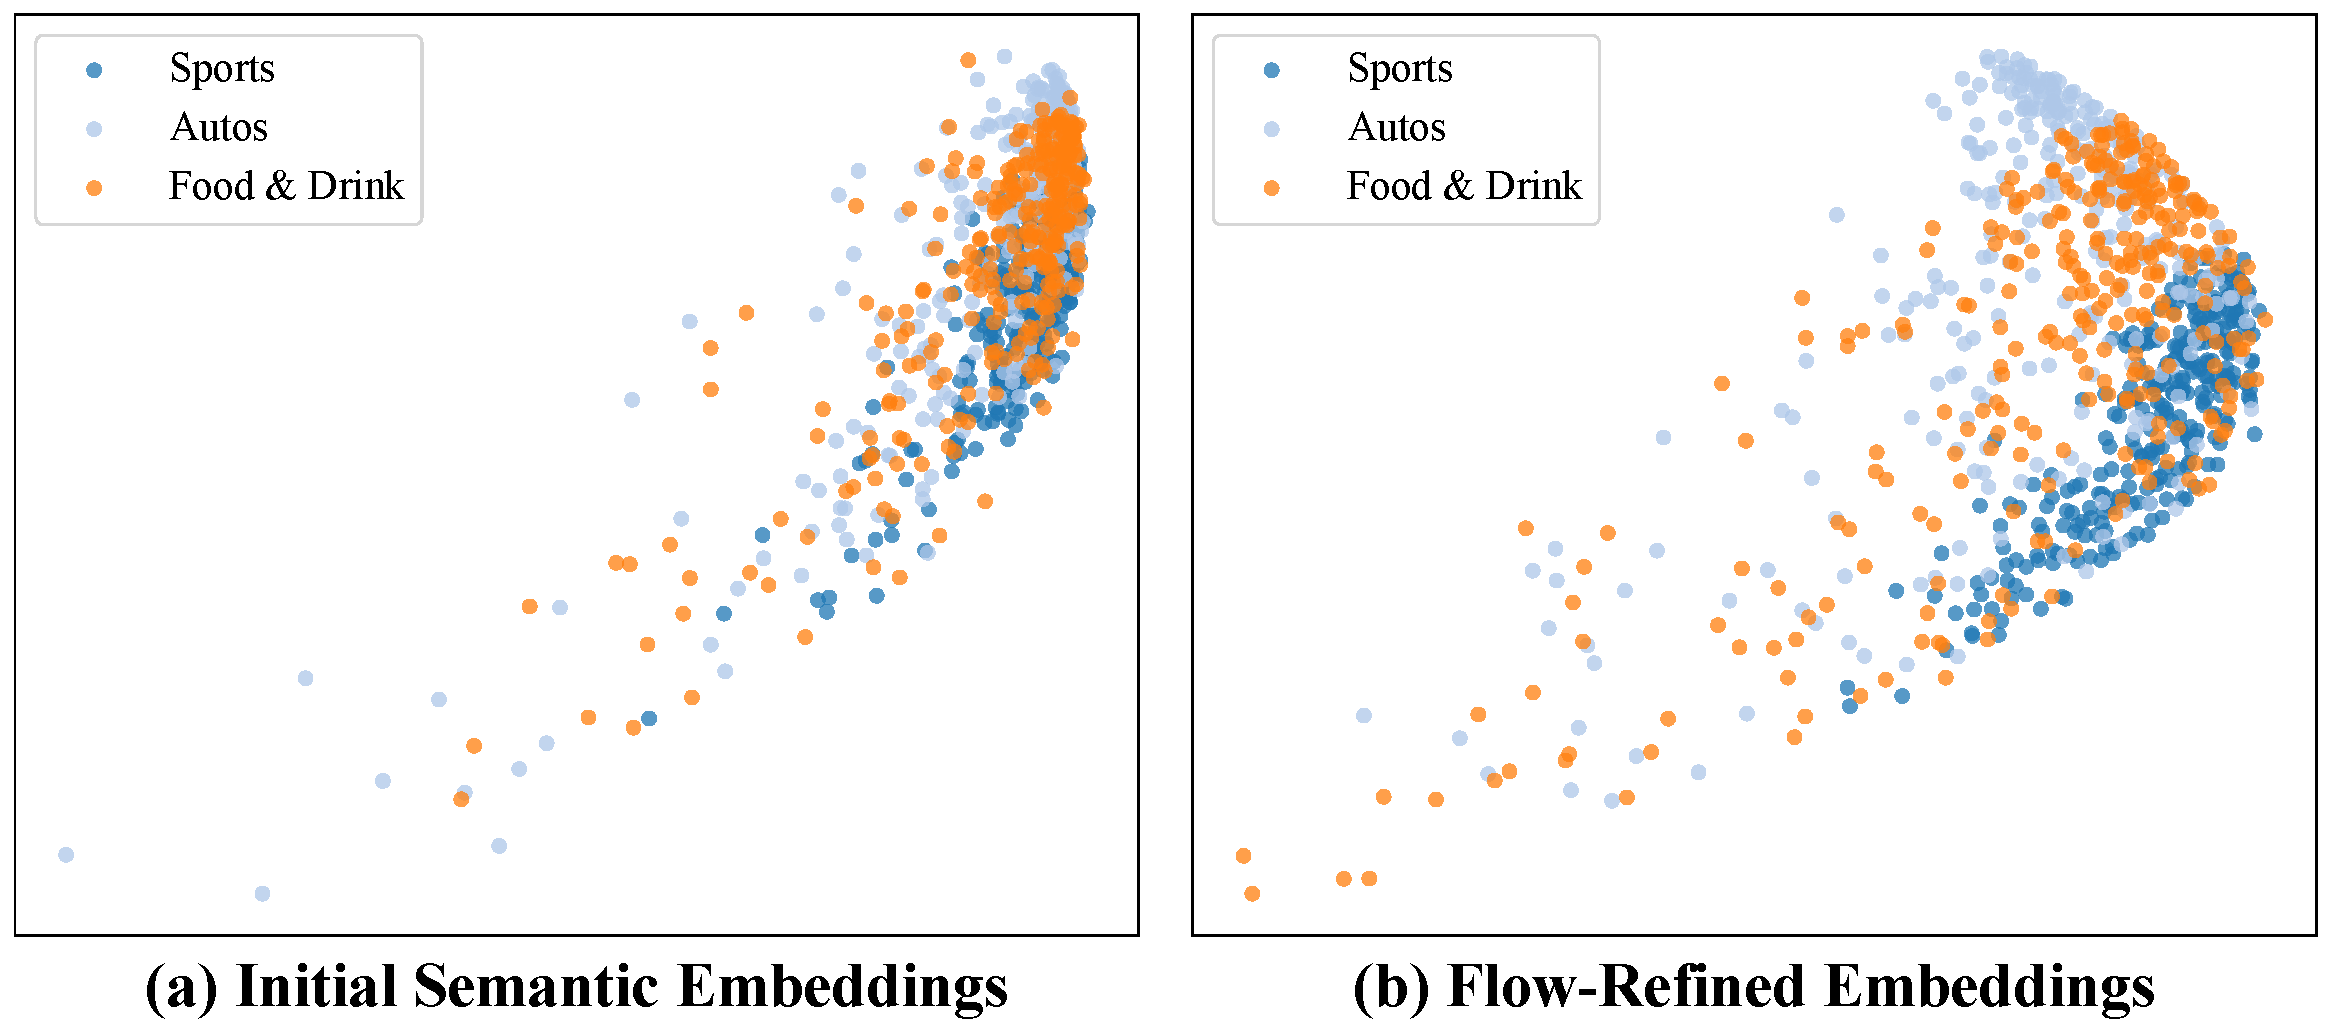
\includegraphics[width=\columnwidth]{image/scatter}
	\caption{Visualization of latent space evolution. (a) Initial embeddings exhibit severe semantic entanglement due to noise. (b) Flow-refined representations form compact, distinct clusters, demonstrating the effective recovery of semantic manifolds.}
	\label{fig:scatter}
\end{figure}



\subsection{Ablation Study (RQ2)}
\subsubsection{\textbf{Key Module Ablation}}
To systematically evaluate the contribution of each component, we compare the full FlowKG with four variants: (1) w/o ESL, removing the Entropy-Guided Structure Learning; (2) w/o DVE, replacing the Decoupled Dual-View Encoder with a coupled GNN architecture; (3) w/o FM, removing the Flow Matching Refinement; and (4) w/o CL, discarding the dual-level CL. For compact presentation, the main text reports three representative datasets in Table~\ref{tab:ablation}, with the complete four-dataset ablation results provided in Appendix~\ref{app:full_ablation}. Figure~\ref{fig:ablation_chart_lastfm} further analyzes the Last-FM mechanism.


Table~\ref{tab:ablation} confirms the full model's superior performance, demonstrating module synergy. First, removing CL causes the most severe degradation (e.g., -34.7\% Recall@20 on MIND), establishing it as a foundational paradigm against data sparsity. Furthermore, the substantial drop without FM verifies its critical role in preventing representation degradation through distributional evolution. Finally, the consistent performance losses without ESL and DVE confirm that filtering structural noise and decoupling views are essential prerequisites for robust representation learning.

Figure~\ref{fig:ablation_chart_lastfm} presents a multi-dimensional ablation study on Last-FM to scrutinize the internal mechanism. The Decoupled Skeleton outperforms the Coupled Skeleton in Recall@20 (0.352 vs. 0.342), empirically validating that strict view decoupling prevents noise propagation. Both additive and subtractive analyses confirm the contribution of each component: adding ESL, FM, or CL individually improves performance, while removing any causes decline. This consistent "building-up" and "stripping-down" evidence robustly verifies that every module in FlowKG distinctively enhances the final performance.

\subsubsection{\textbf{Sensitivity to Key Hyperparameters}}
To investigate the properties of FlowKG, we analyze the impact of three key hyperparameters: the retention rate $\rho$, integration steps $N$, and contrastive temperature $\tau$, as summarized in Figure~\ref{fig:hyperparameter}.


\noindent\textbf{Impact of Retention Rate $\rho$.}
As shown in Figure~\ref{fig:hyperparameter}(a), performance follows a convex pattern across all datasets. Both excessive pruning ($\rho=0.1$) and retaining the full noisy graph ($\rho \to 1.0$) lead to degradation. The optimal sweet spot typically spans from $\rho=0.4$ to $\rho=0.8$, confirming that the Entropy-Guided Structure Learning module successfully identifies a trade-off zone where structural noise is filtered while intrinsic semantic information is preserved.

\noindent\textbf{Impact of Integration Steps $N$.}
Figure~\ref{fig:hyperparameter}(b) demonstrates the remarkable stability of our Flow Matching mechanism. Notably, the model achieves optimal performance within just 1--3 Euler steps, and performance remains consistently stable beyond this point. This implies that the learned vector field constructs a highly straight ODE trajectory in the latent space, allowing the model to jump from noise to the target manifold directly. Consequently, a minimal number of integration steps is sufficient for inference, ensuring maximal computational efficiency without sacrificing accuracy.

\noindent\textbf{Impact of Temperature $\tau$.}
Figure~\ref{fig:hyperparameter}(c) reveals dataset-dependent preferences. Denser datasets like ML-1M benefit from a moderate $\tau$ (e.g., 0.2) to maintain discriminative power. Conversely, on the MIND dataset characterized by extreme interaction sparsity and high-dimensional relations, performance improves monotonically as $\tau$ increases, peaking at the theoretical limit of Mean Difference (MD) loss. This verifies that in scenarios with high sparsity where ``hard negatives'' are likely to be unobserved positives (False Negatives), shifting the objective from local hard-negative discrimination to global representation alignment (via high $\tau$ or MD loss) provides significantly better robustness.

\subsection{Robustness Analysis (RQ3)}


To evaluate robustness against structural perturbations, we inject random KG noise at ratios from 0\% to 20\%. As shown in Figure~\ref{fig:noise_robustness}, FlowKG consistently achieves the best NDCG@20 and degrades more slowly than KMDCL and DiffKG. Removing either ESL or FM reduces robustness, with the gap widening as noise increases. These results confirm that upstream structure filtering and downstream representation refinement provide complementary protection against noisy knowledge.

We further examine robustness under different sparsity conditions on Last-FM. As shown in Figure~\ref{fig:lastfm_sparsity_metrics}, FlowKG maintains consistent advantages across both user and item groups under NDCG@20 and Recall@20, indicating that the proposed decoupled structure learning and flow-based refinement remain effective for sparse recommendation scenarios.

%\begin{figure}[t]
%	\centering
%	\includegraphics[width=\linewidth]{image/case_study} % 插入你的图片文件
%	\caption{Case Study on MovieLens-1M for item \textbf{``Interstellar''}.}
%	\label{fig:case_study}
%\end{figure}

\subsection{Computational Efficiency Analysis (RQ4)}


To investigate the trade-off between recommendation accuracy and resource consumption, we visualize the relationship between NDCG@20, training time (per epoch), and parameter magnitude in Figure~\ref{fig:efficiency_pareto}.
FlowKG demonstrates a superior Pareto efficiency, achieving SOTA performance while maintaining low computational overhead.
In terms of model complexity, FlowKG achieves a significant reduction in parameter count compared to other generative baselines like DiffKG and KMDCL, aligning closely with lightweight discriminative models such as LightKG and KGRec.
This efficiency stems from our design choice to conduct generation in the latent space rather than the graph space.
While KMDCL performs diffusion on the high-dimensional graph structure $\mathbb{R}^{|\mathcal{E}| \times |\mathcal{E}|}$, FlowKG operates strictly within the compact item representation space $\mathbb{R}^{|\mathcal{I}| \times d}$.
This dimensional reduction circumvents the prohibitive parameter costs associated with graph-level generation.
Regarding temporal efficiency, FlowKG consistently ranks in the top tier across diverse datasets.
Unlike SDE-based diffusion models that require computationally expensive stochastic sampling and extensive denoising steps, our Flow Matching framework utilizes a deterministic ODE solver.
This enables rapid convergence during training and efficient inference, successfully reconciling the high expressiveness of generative models with the practicality required for large-scale recommendation.

\subsection{Visual Interpretability of Manifold Evolution (RQ5)}


To intuitively verify the efficacy of the Flow Matching module in rectifying latent representations, we visualize the evolution of item embeddings using Principal Component Analysis (PCA), as depicted in Figure~\ref{fig:scatter}. In the initial state (Figure~\ref{fig:scatter}a), embeddings from distinct categories (e.g., Sports, Autos) exhibit severe semantic entanglement with blurred decision boundaries. This observation confirms that despite the structural pruning, the raw semantic encoder remains susceptible to residual noise, resulting in a dispersed distribution. Conversely, after undergoing the flow-based refinement (Figure~\ref{fig:scatter}b), the representations evolve into compact, well-separated clusters with clear manifold structures. This distinct separation demonstrates that the learned deterministic ODE trajectory successfully acts as a "semantic rectifier," guiding item embeddings from a disordered, noisy distribution to a structured high-density region, thereby significantly enhancing their discriminative power for downstream recommendation.

